\chapter{Dettagli implementativi}
\section{Gestione delle liste}
\begin{itemize}
\diam \textbf{Definizione dei tipi di dato}: \texttt{proxy/types.h}
\diam \textbf{Funzioni utilizzate}: \texttt{proxy/uni\_list.c}
\end{itemize}
La gestione delle liste è effettuata in un modo modulare: le funzioni
\texttt{new}, \texttt{dequeue}, \texttt{remove\_elem}, \texttt{enqueue} e \texttt{push} trattano
esclusivamente la gestione dei tipi di dato delle testate delle liste, che 
verranno utilizzate per gestire i dati compositi di lista che sono utilizzati
in seguito:
\begin{description}
\item[Gestione dei JOB]: \texttt{init\_job\_queue}, \texttt{dequeue\_job}, \texttt{run\_job},
	\texttt{remove\_job}, \texttt{alloc\_new\_job}, \texttt{enqueue\_job}, \texttt{push\_job},
	\texttt{exists\_job\_res}.
\item[Gestione della coda di prefetch]: \texttt{update\_list}.
\end{description}

\section{Gestione della Pool}\label{sec:gdp}
\begin{figure}[!th]
\begin{centering}
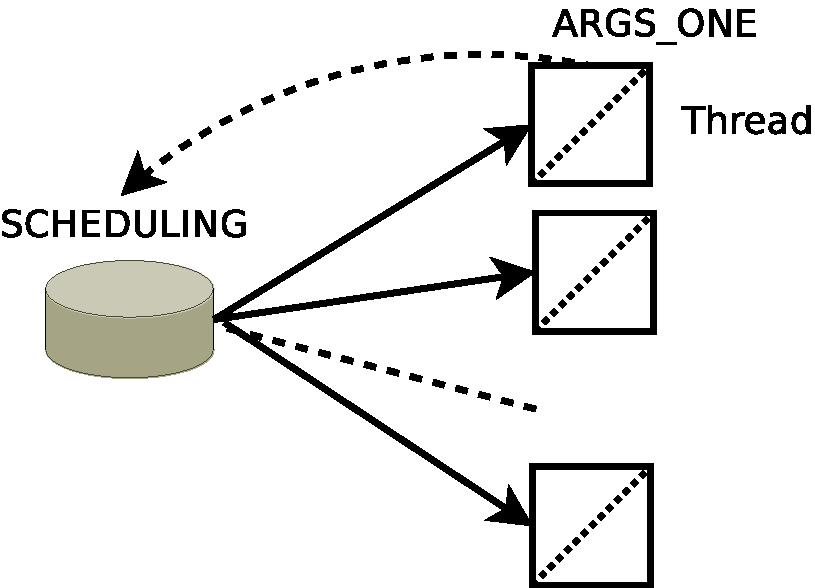
\includegraphics[scale=0.5]{fig/fig01.pdf}
\caption{\textit{Schematizzazione dell'interazione tra thread che attingono le
richieste da una stessa Pool}.}
\end{centering}
\label{fig:gdppw}
\end{figure}
\begin{itemize}
\diam \textbf{Definizione dei tipi di dato}: \texttt{proxy/types.h} 
\diam \textbf{Funzioni utilizzate}: \texttt{proxy/thread\_functs.c}
\end{itemize}
Per quanto concerne la gestione delle Pool, ad ogni thread, all'atto della
creazione, viene passata staticamente per puntatore una propria struttura dati
\texttt{ARGS\_ONE}, all'interno della quale è contenuto un identificatore numerico
del thread correntemente in esecuzione, ed il puntatore per la Pool associata,
del tipo \texttt{SCHEDULING}. Quest'ultima struttura dati, condivisa tra i thread
che si occupano di gestire le richieste in questione, che vengono prelevate dalla
coda di tipo \texttt{LIST}, associata al parametro \texttt{planning}. L'accesso in 
mutua esclusione alla lista, è garantita tramite l'uso del mutex \texttt{qlock},
mentre si garantisce l'attesa senza busy waiting tramite l'attesa su condizione
\texttt{non\_empty}, sulla quale si ci ferma se non ci sono elementi all'interno
della lista (\texttt{qsize==0}).

Come elemento della lista, vengono inseriti un puntatore a funzione, e degli
argomenti che dovranno essere applicate a questa tramite la funzione
\texttt{main\_add\_job}, raccolti all'interno del tipo di dato \texttt{JOB}: la chiamata della funzione
con i suddetti parametri verrà effettuata dallo stesso thread, che ha come 
corpo la funzione ``server'' \texttt{thread\_memento}, che utilizza un particolare
\texttt{ARGS\_ONE} associato al thread.

Qui sotto forniamo un elenco delle Pool che vengono utilizzate all'interno
del nostro progetto:
\begin{itemize}
\item \textit{serverPool}: in questa Pool sono inserite tutte le richieste di 
	ottenimento di una risorsa dal server: queste sono gestite da quattro
	thread, mediante i quali si garantisce che i socket con i quali ci 
	collegheremo per la parte server, siano sempre e soli 4. 
\item \textit{prefetchPool}: in questa Pool vengono memorizzate quali sono le
	risorse da scaricare in prefetch: dato il livello di prefetching della
	risorsa attualmente scandita (es. 1), viene effettuato il parsing della
	risorsa per ritrovare ulteriori elementi in essi contenuti, per poi
	riaccodarli se non si è ottenuto il livello prefissato di prefetching.
	A questa Pool è associato solamente un thread.
\item \textit{cachePool}: in questa Pool sono memorizzate tutte le richieste di
	gestione di ottenimento delle risorse dalla chache: in questa lista
	vengono anche convogliate le gestioni di invio delle informazioni al 
	client, che inizialmente prevedevano eventualmente un'interazione 
	diretta esclusivamente con il server. Questo verrà dettagliato nella
	gestione della connessione in Sezione ~\vref{sec:gdr}.
\end{itemize}

\section{Gestione delle richieste}\label{sec:gdr}
\begin{itemize}
\diam \textbf{Definizione dei tipi di dato}: \texttt{proxy/types.h} 
\diam \textbf{Funzioni utilizzate}: \texttt{proxy/connect.c} 
\end{itemize}
\begin{figure}[!t]
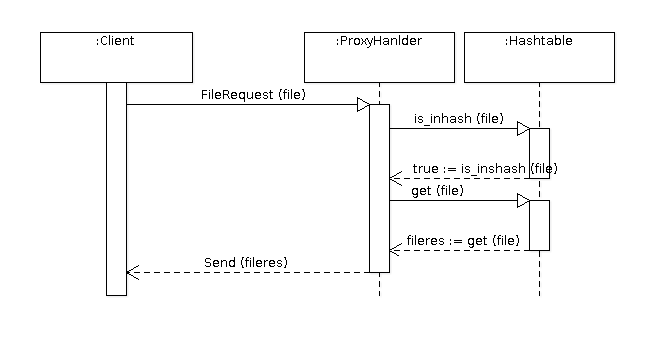
\includegraphics[scale=0.7]{fig/uml/DiagrammadiSequenza13.png}
\caption{\textit{Descrizione dell'interazione Client-Proxy durante una richiesta
di una risorsa presente in cache}.}
\label{fig:dds13}
\end{figure}
\begin{figure}[!t]
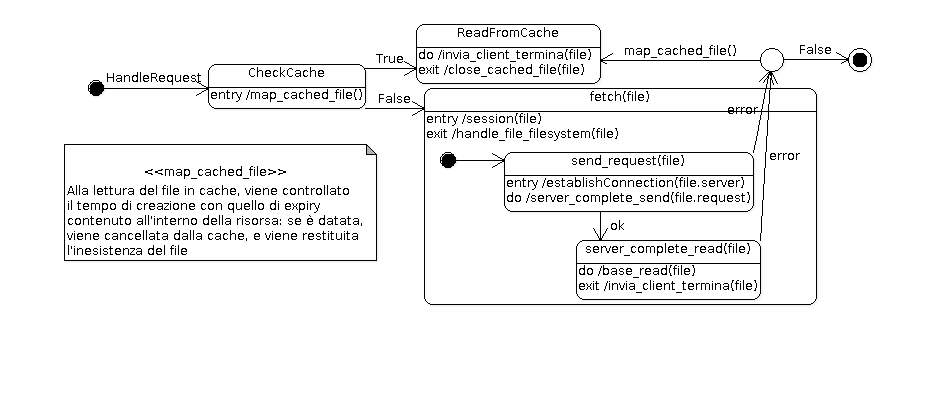
\includegraphics[scale=0.6]{fig/uml/ModelloSenzaNome1.png}
\caption{\textit{Descrizione dell'automa a stati durante la richiesta di una 
risorsa non presente in cache}.}
\label{fig:msn1}
\end{figure}
All'interno del \texttt{main} effettuiamo il controllo se la risorsa sia già presente
in cache: se è presente tale risorsa viene inviata al client, come rappresentato
dall'interazione rappresentata dalla Figura ~\vref{fig:dds13}. Se invece non 
è presente in cache, allora avviene una connessione col server, utilizzando
un'interazione descritta dalla macchina a stati della Figura ~\vref{fig:msn1}.

La descrizione della comunicazione con il client avviene con la funzione
descritta nel file \texttt{proxy/toclient.c}, mentre le funzioni di comunicazione con
il server sono contenute all'interno di \texttt{proxy/toserver.c}: tutte queste
funzioni utilizzano la funzione \texttt{fetch} e \texttt{update\_list}, rispettivamente
per ottenere la risorsa dal server, e per iniziare ad effettuare il prefetch
delle risorse indicate in quella appena scaricata.
Sempre facendo riferimento alla Figura ~\vref{fig:msn1}, possiamo innanzitutto
precisare come tutte le funzioni presenti nello stato \texttt{fetch}, che è di per
se una funzione di \texttt{proxy/toserver.c}, sono descritte all'interno del file
\texttt{proxy/connection}, che si preoccupa di gestire la comunicazione con il
proxy sia per il prefetch, sia per il download da server, su richiesta di un
preciso client.

Le opzioni che vengono impostate sul socket che viene utilizzato per collegarsi
con il server, sono le seguenti:
\begin{itemize}
\diam \texttt{SO\_SNDTIMEO}: se una funzione risulta bloccante, viene settato un
	timeout, oltre al quale tale funzione restituisce l'ammontare delle
	informazioni inviate.
\diam \texttt{TCP\_NODELAY}: disabilita l'algoritmo di Nagle, incrementando 
	conseguentemente la performance, in quanto non consente l'invio di
	frames parziali, in quanto i parti del buffer vengono inviati
	istantaneamente, senza aspettare che il buffer venga sufficientemente
	riempito.
\diam \texttt{SO\_RCVTIMEO}: analoga alla \texttt{SO\_SNDTIMEO}, ma utilizzata per la
	ricezione.
\end{itemize}

\section{Gestione dello stato del Proxy}
\begin{itemize}
\diam \textbf{Definizione dei tipi di dato}: \texttt{proxy/types.h} 
\end{itemize}
Lo stato del proxy viene mantenuto all'interno di due strutture dati: la prima
struttura dati è \texttt{struct proxy}, all'interno della quale vengono salvate le
informazioni attinenti all'accettazione delle richieste da parte di client(s),
l'indirizzo IP e la porta associata, ed il livello di prefetch che viene indicato
all'invocazione del programma.

Lo stato della connessione con il server viene invece mantenuto all'interno
della struttura dati definita \texttt{struct connection}: viene salvato l'indirizzo
IP e porta del server al quale connettersi, la risorsa da richiedere, il numero
dei tentativi effettuati ed il file descriptor del client, al quale alla fine
eventualmente inviare l'informazione, e del server, al quale inviare appunto
la richiesta e ricevere la risposta.
